\documentclass[journal]{IEEEtran}
\usepackage{amsmath,amssymb,graphicx,booktabs,url}
\usepackage[hidelinks]{hyperref}
\newcommand{\BasePCK}{49.14}
\newcommand{\BaseAUC}{0.33796}
\newcommand{\BasePninety}{40.902}
\newcommand{\RawPCK}{47.51}
\newcommand{\RawAUC}{0.33472}
\newcommand{\RawPninety}{41.958}
\newcommand{\CorrPCK}{51.47}
\newcommand{\CorrAUC}{0.35902}
\newcommand{\CorrPninety}{42.085}
\newcommand{\AnchorRaw}{44}
\newcommand{\AnchorRawMed}{7.144}
\newcommand{\AnchorCorr}{50}
\newcommand{\AnchorCorrMed}{5.489}
\newcommand{\StudentDelta}{3.96}
\newcommand{\CILow}{1.83}
\newcommand{\CIHigh}{6.46}

\title{Corrected Pseudo-Label Self-Training for Monocular Pallet Pose Estimation under an Explicit Real-Supervision Budget}
\author{Technical manuscript for author review}
\markboth{Research Manuscript, September 2026; Not Submitted}{Corrected Pseudo-Label Self-Training}
\begin{document}
\maketitle
\begin{abstract}
Synthetic training reduces the need for task-specific real annotations, but self-training can reinforce inaccurate target-domain landmarks. We examine whether correcting pseudo-label coordinates improves monocular pallet pose estimation when the student training conditions are otherwise matched. A frozen PoseFix-derived teacher, adapted using nine real images and 38 manually verified corners with synthetic replay, corrects a synthetic-pallet-pretrained model's predictions. Raw and corrected students share 217 target images, supervision support, initialization, augmentation settings, synthetic replay, and 320 optimizer updates. On 66 directly verified visible development points, correction increases 10-pixel keypoint accuracy from \AnchorRaw{} to \AnchorCorr{} out of 66. On a repeatedly used, recording-disjoint development panel of 128 ordinary-plastic images, corrected versus raw student accuracy improves from \RawPCK{}\% to \CorrPCK{}\%, while fixed-pipeline geometry-reference pose AUC improves from \RawAUC{} to \CorrAUC{}. The synthetic-only baseline obtains \BasePCK{}\% and \BaseAUC{}. Both previously tested learning-rate settings and the available order repeats are retained. Tail error does not uniformly improve, and the pose reference is not independently measured physical ground truth. The evidence supports a scoped development result for corrected-target self-training, not zero-real-label learning, an unseen-session guarantee, or universal large-error recovery.
\end{abstract}
\begin{IEEEkeywords}
Pallet perception, monocular pose estimation, pseudo-labels, self-training, synthetic-to-real adaptation, evaluation provenance.
\end{IEEEkeywords}

\section{Introduction}
An RGB pallet-pose estimator must localize geometric landmarks before recovering object position and orientation. Synthetic images can provide pallet-specific supervision, but real images introduce lighting, occlusion, and viewpoint shifts. A confident predicted box need not imply accurate corners. Consequently, treating every confident prediction as a training target can preserve or amplify localization errors.

The question in this work is deliberately narrower than developing an additional pose architecture: under a disclosed real-supervision budget, are corrected pseudo-label coordinates more useful than the original coordinates for student adaptation? A gain over the original synthetic-only model is insufficient to answer this question. It could instead result from additional optimizer updates, synthetic replay, or a different subset of target images. A useful comparison must hold those factors fixed and compare raw-target and corrected-target students directly.

We close this comparison using an existing matched experiment rather than introduce further modules after inspecting development results. A frozen teacher supplies corrected coordinates, while the student is used without that teacher at inference. We distinguish four questions: label quality on the same verified points; corrected versus raw student performance; practical value over the synthetic-only baseline; and the population and metric scope of the evidence. The contributions are (i) an auditable matched-coordinate self-training comparison with explicit manual supervision, (ii) a joint 2D and fixed-pipeline 6D evaluation with complete denominators, and (iii) an evidence-scope analysis retaining order sensitivity, error tails, and failed examples. Self-training, pose refinement, and PnP are not claimed as new algorithms.

\begin{figure*}[t]
\centering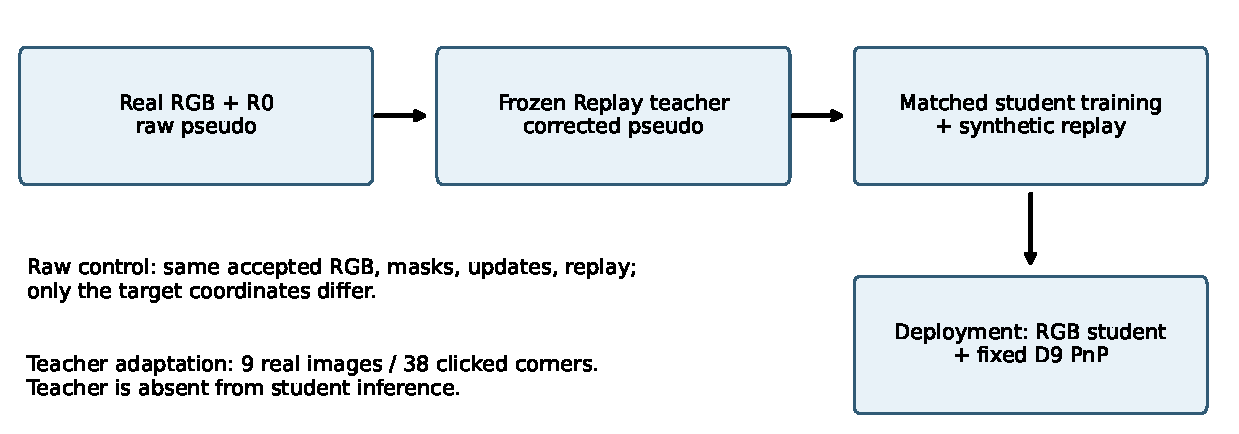
\includegraphics[width=.96\textwidth]{figures/pipeline.pdf}
\caption{The tested information paths. The teacher changes training targets, not deployed student architecture. Both students use the same accepted real images and target-support masks. The final geometry stage is fixed across arms.}
\label{fig:pipeline}
\end{figure*}

\section{Related Work and Scope}
STAC uses confident teacher detections as pseudo-labels and trains a student with augmentation-based consistency\cite{stac}. This motivates separating target quality from student training. Our experiment concerns pallet corner coordinates and matched support, and does not reproduce STAC's object-detection benchmarks or claim its annotation-efficiency results.

PoseFix refines an input human pose from the image and synthesizes training errors using human-pose error statistics\cite{posefix}. Our teacher is a pallet-specific adaptation of this family, not the original human benchmark. It uses pallet landmarks, a synthetic-trained prior, limited real manual coordinates, and synthetic replay. At self-training time the teacher is frozen; there is no human correction of each pseudo-label.

Self6D demonstrates synthetic-to-real pose adaptation with differentiable rendering and unannotated real RGB-D data during adaptation\cite{self6d}. Our tested correction path instead consumes RGB, a predicted box, and predicted landmarks; it does not use a depth sensor or a rendering-based adaptation objective. Registered dimensions and camera intrinsics are used only by downstream geometry and the existing consistency filter.

BOP established evaluation that explicitly addresses object symmetries and pose ambiguity\cite{bop}; subsequent challenge reports distinguish datasets, tasks, and seen versus unseen object conditions\cite{bop2024}. Those distinctions motivate careful reporting here. Our normalized, symmetry-aware cuboid AUC is a repository-specific geometry-reference measurement, not a claim of BOP benchmark equivalence or state-of-the-art performance. None of these prior papers' numerical results is directly compared across incompatible datasets.

\section{Method and Matched Intervention}
\subsection{Baseline and point contract}
The baseline R0 is the existing YOLO26n pallet-pose checkpoint. ``Synthetic-only'' describes its pallet-specific fitting, not the provenance of all pretraining: upstream COCO-pose pretraining is documented. For each image, the fixed inference wrapper returns candidate boxes, scores, and nine landmarks. Corners 0--7 follow the registered cuboid convention; landmark 8 is the existing center. Instance selection and original-image coordinate restoration are unchanged across the comparison. Ground-truth boxes or poses do not choose an inference candidate.

\subsection{Frozen correction teacher}
The teacher is the existing RGB ResNet152 PoseFix-derived pallet network. It was initialized from the synthetic-trained PRIOR1 checkpoint and adapted for 300 updates using eight real and eight synthetic examples per update. The real term supervises only 38 verified manual corners in nine images: three ordinary-plastic night images and six wood-day images. Unknown and PnP-completed points and the center do not supply manual teacher supervision. Frozen batch-normalization statistics and trainable affine parameters follow the original protocol.

Teacher adaptation retains the existing heatmap cross-entropy plus coordinate loss and source replay objective. Real inputs alternate between R0 predictions and manually supported coordinates perturbed with predicted-box-scaled noise. We do not claim that synthetic and real errors have identical distributions. The original fixed final teacher checkpoint is reused without a new fit or development-selected displacement cap. At pseudo-label generation, it consumes only RGB, R0 points, and the predicted crop. It preserves the detection box, score, keypoint confidence, and center, and modifies corner coordinates.

\subsection{Shared image selection and support}
The ordinary-plastic candidate pool contains 1,000 real images outside the evaluation recordings. The existing raw confidence, horizontal-flip agreement, and leave-one-out (LOO) consistency checks retain 259 candidates; applying the frozen teacher and the existing post-correction LOO check retains 249. This pipeline does not imply that an accepted prediction is correct. No new geometric-shape, X-intersection, stability, or threshold sweep is introduced.

Both training arms use this \emph{same} accepted set. A fixed replacement draw produces 512 real slots containing 217 unique images per epoch. For every raw/corrected pair, the box and trusted-keypoint mask are identical. The latter is the intersection of the original target-export validity masks; points outside shared support are ignored in both arms. Thus the controlled contrast concerns corrected versus raw coordinates conditional on a shared teacher-filtered selection policy. It does not estimate the effect of teacher-based selection itself, nor does the raw arm eliminate every influence of the manually adapted teacher.

Let $\tilde{\mathbf y}^{r}_i$ and $\tilde{\mathbf y}^{c}_i$ denote the raw and corrected targets and $m_{ij}$ their common support. With the same augmentation $A$, real batch $B_t$, and synthetic replay batch $S_t$, the intervention is
\begin{equation}
\mathcal L_t^{a}=\mathcal L_{\rm pose}(f_\theta(Ax_i),A\tilde{\mathbf y}^{a}_i;m_i)
+\mathcal L_{\rm source},\quad a\in\{r,c\}.
\end{equation}
This expression describes the existing pose objective and shared support, not a newly designed loss. Identical frozen detector branches retain the same ancillary detection terms. The only altered supervised targets are the real coordinate values.

\subsection{Student training and deployment}
Each student starts independently from the same R0 checkpoint. Only the pose branches and flow parameters are trainable; backbone, neck, box/class branches, and all running buffers remain exactly fixed. Each epoch uses 512 real and 512 synthetic slots; five epochs with batch 16 give 320 updates and 2,560 exposures of each domain. The synthetic pool has 512 unique images and no negative images. Training uses AdamW, cosine decay, and the existing true-ignore keypoint implementation. The checkpoint is the fixed final checkpoint, never an epoch chosen by evaluation performance.

The historical experiment tested learning rates $10^{-4}$ and $10^{-5}$ with matched source-only, raw-target, and corrected-target arms. The latter rate was selected in the earlier reused development study. We disclose that selection, report both settings, and retain both available order repeats at the selected rate. Orders 43 and 44 change sample order; they are not three independent initialization seeds. Corresponding first-batch image-tensor hashes match within each raw/corrected repeat. This is a first-batch check, not a claim that a complete per-step tensor trace was recorded. Table~\ref{tab:fairness} lists the controlled factors.

At deployment, only the student processes RGB. The teacher is absent. The final pose stage uses the same original D9 width/depth hypothesis selector for every arm and solves from corners 0--7. Landmark 8 remains part of the original selector residual; that known design choice is held fixed rather than altered to favor an arm. No trained model-specific router, reference-dependent oracle, or additional inference-time correction enters the main comparison.
\begin{table}[t]
\centering\small
\caption{Matched coordinate intervention. Shared image membership is conditioned on the same raw-plus-refined filter acceptance, so this is not a comparison of different selection policies.}
\label{tab:fairness}
\resizebox{\columnwidth}{!}{%
\begin{tabular}{lr}
\toprule
Contract & RAW and corrected \\
\midrule
Initialization & Same R0 checkpoint \\
Trainable state & Pose branches and flow only \\
Real RGB & 217 identical unique images \\
Real/synthetic exposure & 2560 / 2560 each \\
Synthetic pool & 512 identical images; no negatives \\
Supervised support & Identical raw/ref confidence intersection \\
Optimizer / updates & AdamW / 320 \\
Learning rate & 1e-5 main; 1e-4 sensitivity \\
Augmentation / seed & Same settings / 42 \\
Checkpoint choice & Fixed final last.pt \\
Teacher supervision & 9 images / 38 manual corners \\
Only changed target & Supervised pseudo coordinates \\
\bottomrule
\end{tabular}}
\end{table}


\section{Evaluation Protocol}
\subsection{Populations and reference provenance}
The main panel comprises 128 ordinary-plastic images from seven recording groups, with 29 Clean, 21 Moderate-occlusion, and 78 Severe-occlusion images. Its recording groups do not overlap the pseudo-label training pool or the teacher's manual-training sessions, including recorded aliases. Nevertheless, this is repeatedly inspected development data, not independent confirmation. The historical full 194-image plastic panel included three teacher-training images; that aggregate is not substituted for the present comparison. The 300-image mixed-material panel is not pooled with these denominators.

Label-quality evaluation uses 66 directly verified visible corners in 16 images within the 128-image panel. The frozen FINAL\_V2 reference retains only manually clicked, directly visible points after human metadata QA. Scoring uses fixed native point identity, without choosing a symmetry permutation. Missing points receive the native image diagonal as error. This is a selected, labeled development proxy for pseudo-label quality; it cannot establish the unknown accuracy of every accepted unlabeled adaptation image or the accuracy of hidden corners.

The full-panel legacy labels contain mixed point provenance. Their geometry-resolved poses combine image annotations, intrinsics, and registered dimensions and are not external physical 6D measurements. Because image references and pose references are related, agreement on both does not constitute two independent forms of metrological validation.

\subsection{Metrics and fixed denominators}
The main localization metric is PCK10, the fraction of all supported corners within 10 original-image pixels. PCK5 and PCK20, median error, P90, and errors above 20 pixels are also retained. These pixel thresholds are transparent operating tolerances for this dataset, not asserted universal pallet or robotics standards. Full-panel scoring uses one permitted whole-object symmetry permutation, not independent point-wise nearest matches. Fixed-identity results are retained separately. All 128 images contain detections, but only 120 meet the unchanged box-IoU matching gate of 0.5. Full-denominator PCK includes penalties for the remaining images over 985 supported corners; matched median/P90 uses 931 observed corners. Neither difficult frames nor failures are removed from PCK.

Final pose reporting includes coverage, width/depth-axis correctness, rotation and yaw error, translation error in centimeters, cuboid IoU3D, and normalized ADDsym AUC. The latter integrates the unchanged symmetry-aware error-threshold accuracy curve up to 0.1 object diameter. Failed poses count against AUC; every arm yields a pose for all 128 images here. An axis-correct hypothesis need not have accurate full rotation, and favorable AUC need not improve the median of every pose statistic.

The primary 2D contrast isolates coordinate learning; the common final pose pipeline tests its downstream value. Model-conditioned selectors and nondeployable reference oracles remain separate historical extensions. No new latency or operational-safety claim is inferred from these accuracy measurements.

\subsection{Uncertainty and retrospective disclosure}
We report paired per-frame changes, correct/incorrect corner transitions, every recording group, both learning-rate settings, and all order repeats. A 10,000-draw recording-cluster bootstrap describes PCK10 differences. Corners are not treated as independent experimental replicates. With only seven reused recording groups and historical configuration search, these intervals are exploratory and not search-adjusted. The present closure fixes the scope before new re-evaluation, but is not a prospective preregistration of the original experiments.

\section{Results}
\subsection{Q1: Does the teacher improve target quality?}
On the same verified points, PCK10 increases from \AnchorRaw/66 to \AnchorCorr/66, and median error decreases from \AnchorRawMed{} to \AnchorCorrMed{} pixels (Table~\ref{tab:quality}). The P90 and count of errors above 20 pixels also decrease. This supports improved visible-point quality on this proxy, not perfect correction or unmeasured accuracy on all training targets. Figure~\ref{fig:pseudo} includes both an improvement and a deterioration selected from the actual paired errors.
\begin{table*}[t]
\centering\small
\caption{Pseudo-label quality on 66 verified visible points in 16 reused DEV images; fixed native identity. A labeled proxy, not accuracy measured on unlabeled adaptation images.}
\label{tab:quality}
\resizebox{\textwidth}{!}{%
\begin{tabular}{lrrrrrrr}
\toprule
Output & Points & PCK5 \% & PCK10 \% & PCK20 \% & Med px & P90 px & Above20 \\
\midrule
Synthetic-only R0 & 66 & 21/66 (31.82) & 44/66 (66.67) & 60/66 (90.91) & 7.144 & 18.390 & 6 \\
Frozen Replay teacher & 66 & 30/66 (45.45) & 50/66 (75.76) & 63/66 (95.45) & 5.489 & 13.759 & 3 \\
\bottomrule
\end{tabular}}
\end{table*}

\begin{figure*}[t]
\centering
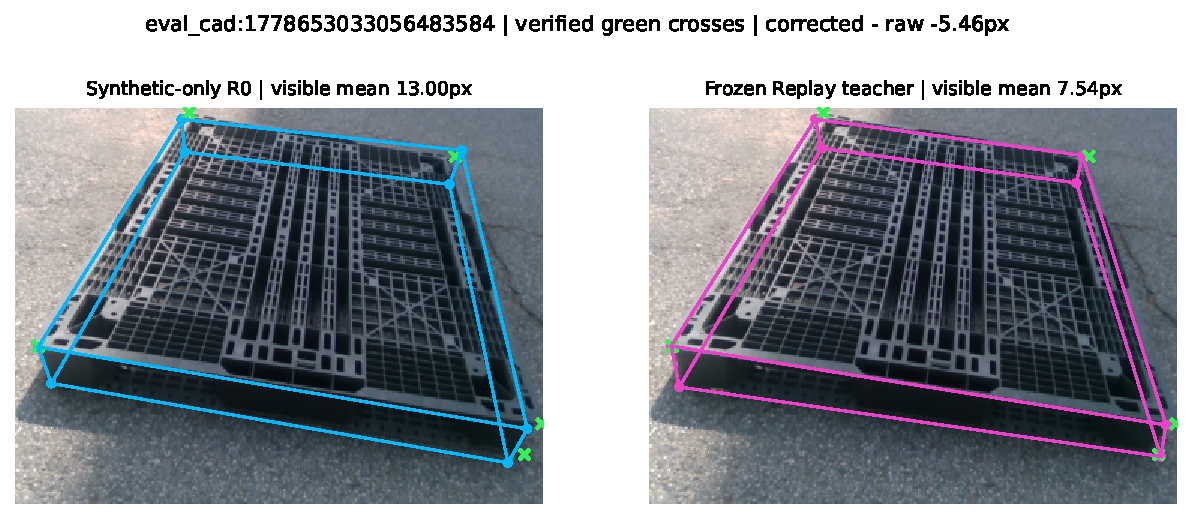
\includegraphics[width=.72\textwidth]{figures/pseudo_quality_01.pdf}\\
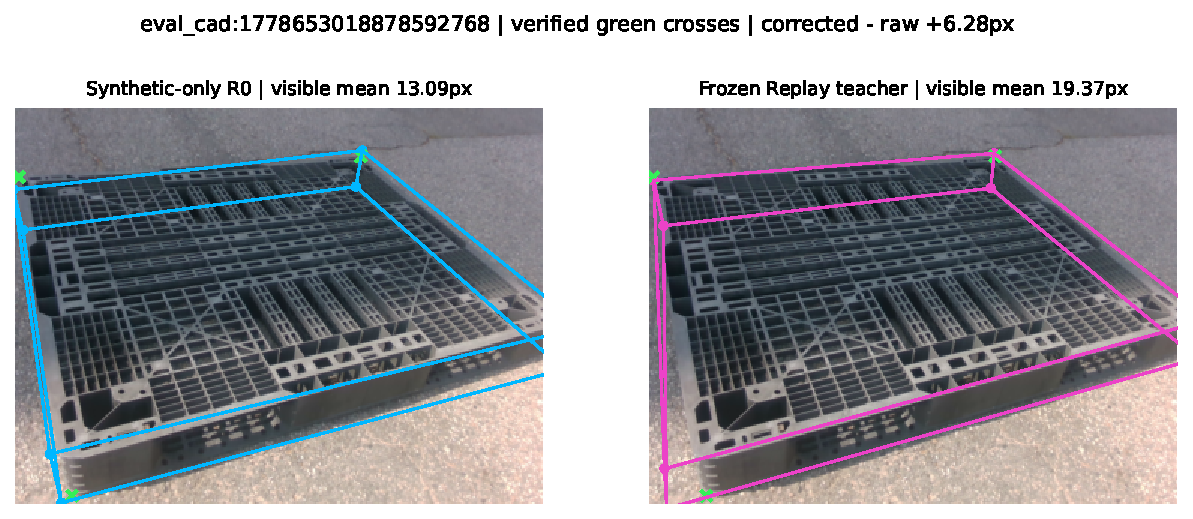
\includegraphics[width=.72\textwidth]{figures/pseudo_quality_04.pdf}
\caption{Frozen raw versus corrected pseudo-label examples: one favorable and one unfavorable visible-point case. Green crosses are directly verified visible references. The actual images and predictions are reused, not synthesized; examples are selected post hoc for explanation and do not determine inference or aggregate membership.}
\label{fig:pseudo}
\end{figure*}

\subsection{Q2: Does corrected-target training improve the student?}
At the previously selected learning rate, corrected-target training raises PCK10 from \RawPCK{}\% to \CorrPCK{}\% (Table~\ref{tab:main2d}), a \StudentDelta{} percentage-point difference. The descriptive recording-bootstrap interval is [\CILow{},\CIHigh{}] percentage points. The paired mean scored frame error improves on 92 images, worsens on 28, and is unchanged on eight. At the 10-pixel boundary, 51 corners become correct and 12 become incorrect. The eight unchanged frame scores include detection-gate penalty ties; they are not necessarily identical predicted coordinates. No raw corner above 20 pixels becomes correct within 10 pixels in this main student contrast. The gain should therefore not be described as successful general large-error recovery.

The pose stage also improves under identical selection and solver code: ADDsym AUC changes from \RawAUC{} to \CorrAUC{} (Table~\ref{tab:main6d}). This is a final-pipeline result, not an oracle choice among poses. The other historical learning rate and both order repeats retain a favorable corrected-versus-raw direction for pooled PCK10 and AUC (Table~\ref{tab:controls}). They support consistency within the explored settings, not independent dataset replication.

Importantly, on the smaller manually reverified subset the two students tie at 43/66 PCK10, compared with R0's 44/66 (Table~\ref{tab:verified}). Corrected-student PCK20 and P90 improve there, but its median is slightly worse than the raw student's. Thus the full-panel PCK10 gain is not reproduced at that threshold on this visible-only reference. Teacher quality and student improvement are distinct measurements; the favorable teacher result cannot replace this student check.
\input{generated_tables/TABLE2_main_2d.tex}
\begin{table*}[t]
\centering\small
\caption{Final 6D under the SAME frozen D9 selector and corner-only solver. Reference is geometry-derived, not independently measured physical pose.}
\label{tab:main6d}
\resizebox{\textwidth}{!}{%
\begin{tabular}{lrrrrrrr}
\toprule
Arm & Pose & Axis & R deg & Yaw deg & t cm & IoU3D & ADDsym AUC \\
\midrule
R0 & 128/128 & 83/128 & 3.530 & 2.756 & 9.353 & 0.5865 & 0.33796 \\
RAW\_LR5 & 128/128 & 81/128 & 3.942 & 2.626 & 9.226 & 0.5808 & 0.33472 \\
REF\_LR5 & 128/128 & 82/128 & 3.766 & 2.550 & 9.186 & 0.5928 & 0.35902 \\
\bottomrule
\end{tabular}}
\end{table*}


\subsection{Q3: What is added beyond synthetic-only R0?}
R0 obtains \BasePCK{}\% PCK10 and \BaseAUC{} pose AUC, compared with \CorrPCK{}\% and \CorrAUC{} after corrected-target self-training. The raw-target student is worse than R0 on those pooled metrics, so the result is not simply a benefit of any self-training. The source-only update controls are included to expose effects of additional source optimization. No detector improvement is claimed: detector boxes, scores, and candidate order remain exactly unchanged.

There is no all-metric dominance. Matched-corner P90 is \BasePninety{} pixels for R0, \RawPninety{} for the raw student, and \CorrPninety{} for the corrected student. The corrected model's median rotation error and axis count do not surpass R0. AUC improves despite a worse median normalized ADDsym error, reflecting different regions of the error distribution. These are observable trade-offs, not omitted measurements.

\subsection{Q4: Where does the result hold?}
Table~\ref{tab:severity} retains all difficulty levels. Corrected versus raw PCK10 and AUC improve in all three strata at LR5, but corrected versus R0 Moderate PCK10 is lower. Severe pose AUC changes little relative to R0, and its median translation error remains worse. Recording-wise results are retained in Table~\ref{tab:recordings}; small groups must not be interpreted as precise new-domain estimates. The strongest claim is pooled and scoped to these ordinary-plastic development recordings.
\input{generated_tables/TABLE3_severity.tex}
\begin{figure*}[t]
\centering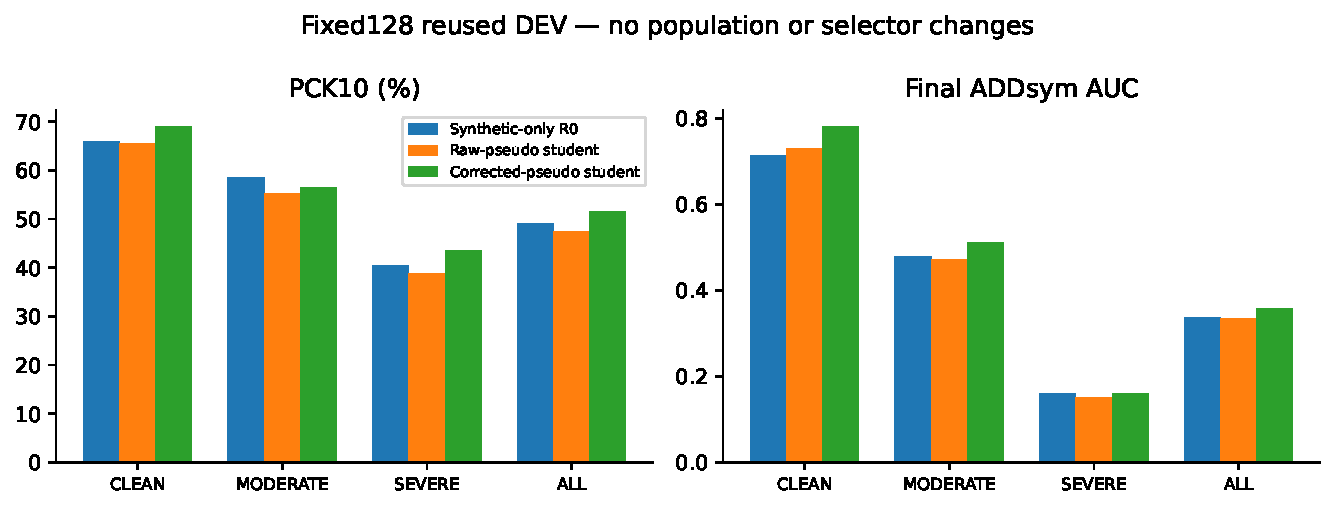
\includegraphics[width=.9\textwidth]{figures/severity.pdf}
\caption{All pre-existing severity strata, under the same evaluation contract. Pooled gains do not establish uniform tail-error recovery or independent generalization.}
\end{figure*}

\section{Limitations and Evidence Closure}
First, the teacher uses real manual supervision. Our intervention is conditional on nine adaptation images and 38 corners, as well as a shared teacher-filtered training selection. We do not claim zero real labels, superiority to directly spending the same annotation budget on the student, or a measured reduction in human annotation time. The 66 verified evaluation points are additional human effort and never student-training targets. Generic pretraining and earlier development annotation/inspection also remain part of the full project history.

Second, the real adaptation data and evaluation recordings are disjoint, but the evaluation panel has been repeatedly used for method development. The LR5 setting was chosen in that history. Session-disjoint fitting does not undo that repeated inspection. The reserve provenance audit found no currently certified untouched, labeled confirmation panel; filename labels such as FINAL are not proof of independence. We therefore close a development-only manuscript without reporting an independent-confirmation number. A future untouched confirmation should be evaluated once with the locked pipeline, without using it to select the learning rate, filters, or checkpoint.

Third, the selected visible-point reference and mixed-provenance full-panel reference answer different questions. Neither proves hidden-corner accuracy or independent physical pose accuracy. The main result covers ordinary rectangular plastic, not wood or square green pallets. Related Clean19 occlusion-transfer, manually supervised hard-image, and model-specific selector studies involve different budgets or interventions and are treated only as extensions, not added to this causal contrast.

Finally, the pose-head-only matched experiment does not show that arbitrary whole-model fine-tuning or other teacher architectures will improve. P90 and severe errors remain unresolved. Figure~\ref{fig:students} explicitly includes a worsened case and a low-change case. No additional architecture, loss, selector sweep, or annotation round is triggered to remove these limitations. The appropriate next action is manuscript review and, if required, independent confirmation, rather than open-ended method search.

\section{Conclusion}
With identical target images, supervision masks, initialization, augmentation settings, synthetic replay, and update budget, corrected pseudo-label coordinates improve the observed ordinary-plastic student's pooled keypoint accuracy and fixed-pipeline pose AUC relative to raw pseudo-labels. The same metrics also improve relative to the synthetic-pallet-only baseline, under an explicit nine-image, 38-corner teacher-adaptation budget. The result is supported within reused development data and does not establish uniform tail recovery or independent physical-pose generalization. This scoped conclusion closes the central experiment without requiring every auxiliary metric to improve.

\appendices
\section{Sensitivity, Failure Cases, and Reproduction}
Table~\ref{tab:controls} contains all twelve existing student fits; no new fitting was performed during evidence closure. Table~\ref{tab:recordings} retains every evaluation recording. The repository package provides checkpoint and source hashes, full optimizer and augmentation arguments, split and target-support contracts, common-selector predictions, numerical provenance for every table, and the paired audit. Exact private RGB/annotation access is needed for full regeneration; hash manifests alone are not a public dataset release. Code and report location: \url{https://github.com/CanelE452/pallet-6d-pose}, namespace \texttt{pallet\_selftraining\_paper\_closure\_v1}.
\begin{table}[t]
\centering\small
\caption{Complete historical grid and order sensitivity. SYN is additional source-only training. ORDER43/44 change data order, not initialization seed. No best-repeat selection.}
\label{tab:controls}
\resizebox{\columnwidth}{!}{%
\begin{tabular}{lrrr}
\toprule
Arm & PCK10 \% & P90 px & ADDsym AUC \\
\midrule
R0 & 49.14 & 40.902 & 0.33796 \\
SYN\_LR4 & 47.41 & 42.356 & 0.33443 \\
RAW\_LR4 & 47.31 & 42.343 & 0.34073 \\
REF\_LR4 & 50.76 & 42.569 & 0.35311 \\
SYN\_LR5 & 48.63 & 41.776 & 0.33895 \\
RAW\_LR5 & 47.51 & 41.958 & 0.33472 \\
REF\_LR5 & 51.47 & 42.085 & 0.35902 \\
SYN\_ORDER43 & 48.93 & 41.762 & 0.33945 \\
RAW\_ORDER43 & 48.32 & 41.808 & 0.33799 \\
REF\_ORDER43 & 51.78 & 42.653 & 0.36100 \\
SYN\_ORDER44 & 48.83 & 41.760 & 0.33994 \\
RAW\_ORDER44 & 47.72 & 41.951 & 0.33684 \\
REF\_ORDER44 & 51.27 & 42.294 & 0.35880 \\
\bottomrule
\end{tabular}}
\end{table}

\begin{table}[t]
\centering\small
\caption{Every reused recording group, including small or adverse groups. Percentages are descriptive, not independent frame trials.}
\label{tab:recordings}
\resizebox{\columnwidth}{!}{%
\begin{tabular}{lrrrrr}
\toprule
Recording & N & Raw PCK10 & Corr PCK10 & Raw AUC & Corr AUC \\
\midrule
REC\_007 & 33 & 47.71 & 49.24 & 0.08383 & 0.09958 \\
REC\_021 & 18 & 39.71 & 45.59 & 0.80000 & 0.81567 \\
REC\_022 & 16 & 32.79 & 36.89 & 0.22866 & 0.24034 \\
REC\_025 & 27 & 38.07 & 44.16 & 0.36820 & 0.38743 \\
REC\_027 & 12 & 26.09 & 36.96 & 0.14642 & 0.12592 \\
REC\_041 & 10 & 71.25 & 71.25 & 0.23680 & 0.31110 \\
REC\_044 & 12 & 96.88 & 96.88 & 0.66275 & 0.75483 \\
\bottomrule
\end{tabular}}
\end{table}

\begin{table}[t]
\centering\small
\caption{Verified-visible student sensitivity: both students tie at PCK10; the legacy-panel gain is not reproduced at this threshold on the small manually reverified subset. Same66 points, fixed identity.}
\label{tab:verified}
\resizebox{\columnwidth}{!}{%
\begin{tabular}{lrrrr}
\toprule
Arm & PCK10 & PCK20 & Median px & P90 px \\
\midrule
R0 & 44/66 & 60/66 & 7.144 & 18.390 \\
RAW\_LR5 & 43/66 & 60/66 & 7.046 & 19.574 \\
REF\_LR5 & 43/66 & 63/66 & 7.097 & 17.343 \\
\bottomrule
\end{tabular}}
\end{table}

\begin{figure*}[t]
\centering
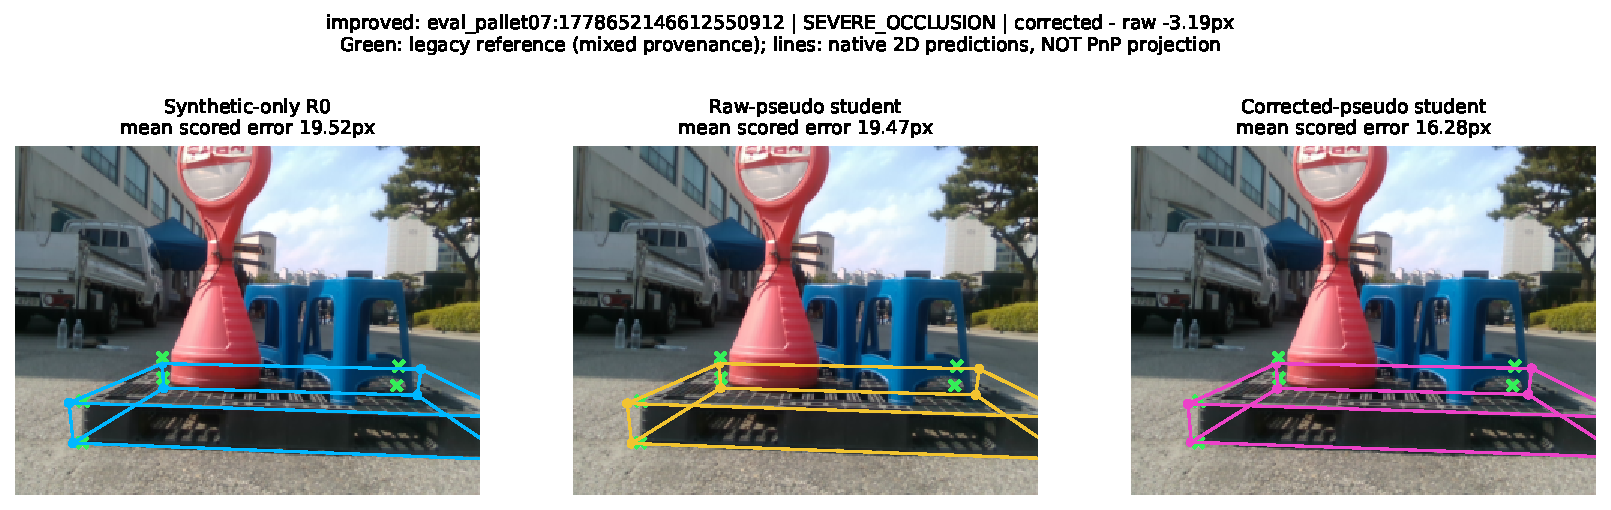
\includegraphics[width=.96\textwidth]{figures/student_01_improved.pdf}\\
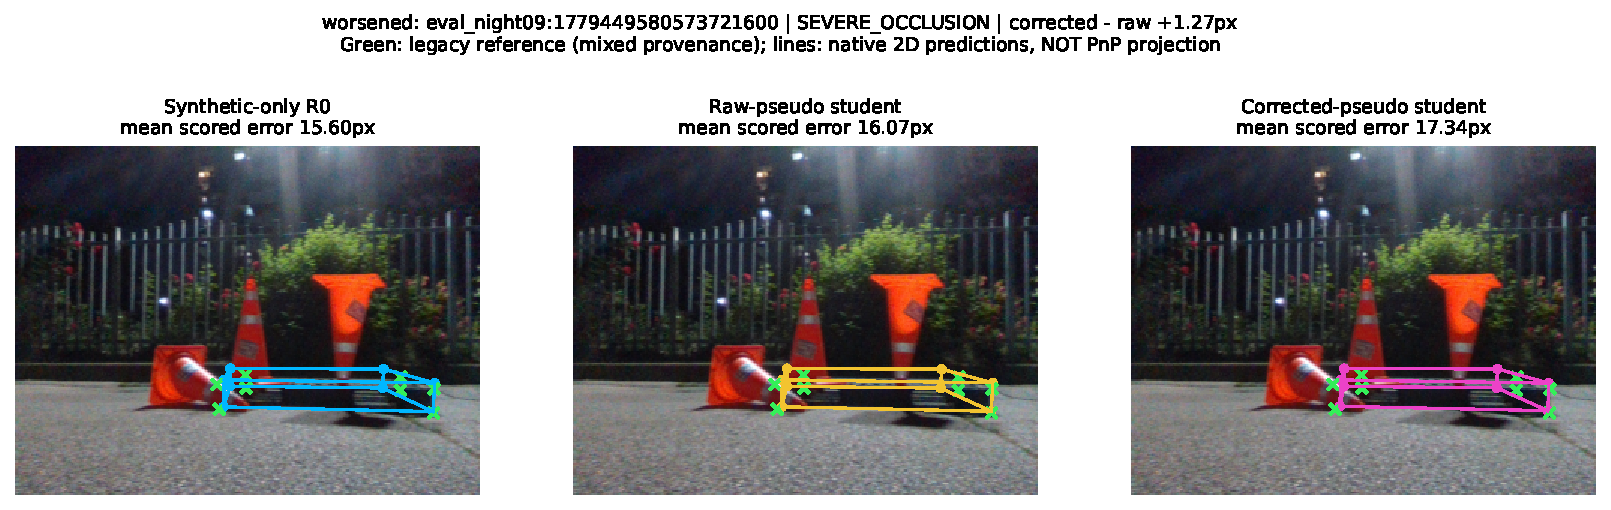
\includegraphics[width=.96\textwidth]{figures/student_06_worsened.pdf}
\caption{Actual student examples with strong improvement (top) and deterioration (bottom) in mean scored corner error. The cyan/yellow/magenta native prediction overlays are R0/raw/corrected students, respectively; green crosses are legacy references of mixed provenance. These are raw 2D predictions, not PnP reprojections. Full-panel error scoring uses the frozen whole-object symmetry contract; image lines retain native identity.}
\label{fig:students}
\end{figure*}
\begin{figure*}[t]
\centering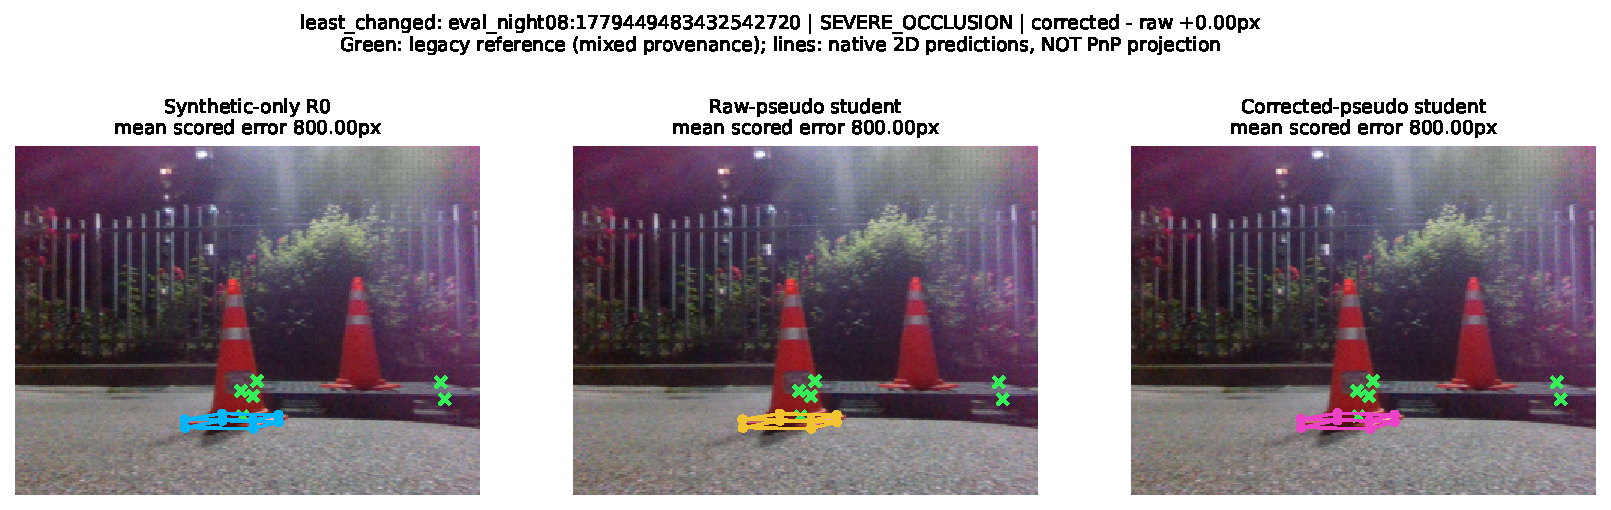
\includegraphics[width=.96\textwidth]{figures/student_07_least_changed.pdf}
\caption{A low-change scored case retained alongside favorable and unfavorable examples. Identical detection penalties can yield an unchanged score even if point coordinates move; no inference correction was chosen using these references. The Markdown report contains all 13 paired example images.}
\end{figure*}
\bibliographystyle{IEEEtran}
\bibliography{references}
\end{document}
